\documentclass[a4paper, 11pt]{book} % Définition de la classe du document courant
%% Packages
\usepackage[utf8]{inputenc}
\usepackage[T1]{fontenc}

\usepackage[english, frenchb]{babel}

\usepackage{natbib}
\bibliographystyle{apalike}

\usepackage[hidelinks]{hyperref}

\usepackage{xcolor}

\hypersetup{
    pdftitle=Doc \LaTeX,
    pdfauthor=A. Mhamdi,
    pdfsubject=Savoir \'ecrire avec \LaTeX,
    colorlinks,
    linkcolor={blue!80!red},
    citecolor={red!80!blue}
}

\usepackage[Lenny]{fncychap}

\usepackage{fancyhdr}
\pagestyle{fancy}

\fancyhf{}

\fancyhead[RE, LO]{\bfseries\normalsize\thepage}

\fancyhead[LE]{\bfseries\nouppercase\leftmark}
\fancyhead[RO]{\bfseries\nouppercase\rightmark}

\usepackage{graphicx}
\graphicspath{{Images/}}

\usepackage{lipsum} 

\title{Mon premier document avec \LaTeX} % Le premier argument. Il s'agit du titre de mon document.
\author{Moi même}
\date{}

\begin{document}
	
\selectlanguage{french}

\maketitle
\thispagestyle{empty}

\frontmatter

% Dédicaces
% Remerciements

\pagenumbering{Roman}

\tableofcontents
\listoffigures
\listoftables

\mainmatter

\chapter*{Introduction générale}
\addcontentsline{toc}{chapter}{\numberline{}Introduction générale}
\markboth{Introduction générale}{Introduction générale}

Les travaux de la présente ***

\chapter{Manipulations générales}
Les travaux de \cite{einstein} ont discuté beaucoup de choses. 

Une documentation complète sur l'usage de \LaTeX\ est accessible à partir des références \cite{latexcompanion, Knuth1984}.

Une image exemple d'une calculatrice scientifique est donnée par la figure~\ref{fig:MyFig}.

\begin{figure}[tbh]
	\centering
	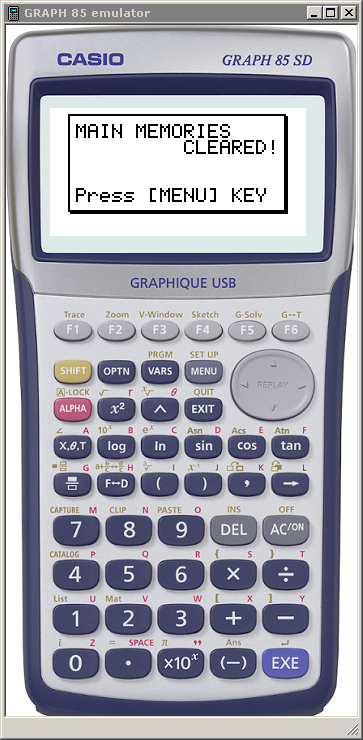
\includegraphics[width=4.25cm, height=7cm]{Casio}
	\caption{Exemple d'une calculatrice scientifque.}
	\label{fig:MyFig}
\end{figure}

La table~\ref{tab:MonTableau} montre un exemple.

\begin{table}
\centering
\caption{Mon tableau.}
\label{tab:MonTableau}
 \begin{tabular}{|l|c|r|}
	\hline
	A & 1 & \begin{tabular}{cc}
		a & b \\
		\hline
		c & d \\
	\end{tabular}
	\\
	B & 2 & \\
	C & 3 & \\
	D & 4 & \begin{tabular}{c}
		\hline
		x \\
		y \\
		z \\
		\hline
	\end{tabular}
	\\
	\hline
\end{tabular}
\end{table}

\cite{RICHARD20031667}

\textbf{AAAAAAAA}\textit{AAAAAAAAA}\underline{AAAAAAAAAAA}\textcolor{blue}{AAAAAA}AAAAAAAA


\chapter{Mon deuxième chapitre}
\section{Ma première section} 
\lipsum[1]

\subsection{Ma sous-section 1.1}
\lipsum[1]
\subsubsection{Ma sous-sous-section 1.1.1}
\lipsum[1]
\subsubsection{Ma sous-sous-section 1.1.2}
\lipsum[1]
\subsection{Ma sous-section 1.2}
\lipsum[1]
\subsubsection{Ma sous-sous-section 1.2.1}
\lipsum[1]
\subsubsection{Ma sous-sous-section 1.2.2}
\lipsum[1]

\section{Ma deuxième section}
\lipsum[1-3]


\chapter*{Conclusion générale}
\addcontentsline{toc}{chapter}{\numberline{}Conclusion générale}
\markboth{Conclusion générale}{Conclusion générale}
\lipsum[1-5]

\backmatter

% Charger les références bibliographiques
\phantomsection
\addcontentsline{toc}{chapter}{\numberline{}Bibliographie}
% \selectlanguage{english}
\bibliography{Biblio/MyBib}

\end{document} 